% to do

Die elektrische Energieversorgung wird mittels getrennter Speisungen erstellt,
da sowohl digitale Logik als auch Leistungselektronik vorhanden ist. Diese
haben sehr unterschiedliche Anforderungen an die Energieversorgung, welche
mittels getrennter Speisungen effektiv zu erfüllen sind.

\paragraph{Spannungsversorung digitaler Komponenten}
Die digitalen Komponenten der Vorrichtung beinhalten primär das
Raspberry Pi und das Freedomboard. Das Freedomboard ist mittels eines USB
Kabels an das Raspberry Pi angeschlossen. Somit ist dieses durch den
USB Port des Raspberry Pi versorgt.

Das Raspberry Pi ist jedoch extern gespiesen. Hierzu wird ein
handelsübliches Steckernetzteil verwendet, welches über den Micro-USB
Anschluss des Raspberry Pi angeschlossen ist.

\paragraph{Spannungsversorgung der Leistungselektronik}
Die Spannungsversorgung der Leistungselektronik inklusive
der Motoren kann aktuell noch nicht definiert werden, da dies stark von den
eingesetzten Motoren abhängt. Hierbei gibt es je nach Motorentyp verschiedene
Anforderungen an die Quellen. Die Tabelle \ref{tab:power-requirement} zeigt
realistische Daten für die jeweiligen Motorentypen welche zum Einsatz kommen.

\begin{table}[h!]
	\centering
	\begin{tabular}{l r r r}
		Motorentyp
			& $U$ [V]
			& $I$ [A] 
			& $P$ [W] \\
		\hline
		Schrittmotor
			& 40
			& 2 
			& 80 \\
		Brushlessmotor
			& 12
			& 40
			& 480 \\
		Gleichstrommotor
			& 12
			& 5
			& 60 \\
	\end{tabular}
	\caption{Übersicht typischer Quellenanforderungen für verschiedene
		Motorentypen}
	\label{tab:power-requirement}
\end{table}

Kritisch sind die Anforderungen des Brushlessmotors, welcher hohe Ströme
fordert. Dies verhindert den Einsatz einfacher Netzteile sondern verlangt
nach speziellen Lösungen. Quellen welche solch hohen Ströme liefern können,
sind typischerweise Batterien, wenn ein kurzzeitiger Einsatz genügt für die
geplante Anwendung. Dies ist bei der automatischen Ballwurfmaschine der
Fall. Für Anwendung welche eine längere Betriebszeit verlangen, ist der
Einsatz von Leistungsstarken Netzteilen notwendig, welche typisch für die
geplante Anwendung hin entwicklet werden.

Für den Einsatz von Batterien spricht die hohe Strombelastbarkeit und die
Gewichtsreduktion, da diese nicht zum Gewicht der Wurfmaschine mitgerechnet
werden. Ebenso ist das Preis/Leistungsverhältnis besser für
hohe Ströme im Vergeich zu Netzteilen. Nachteilig ist, dass die Betriebszeit
der Wurfmaschine stark limitiert ist. Zudem erfordert der Einsatz von
Batterien auch entsprechende Ladegeräte, welche die Kostenersparnis von
Batterien direkt wieder ausgleichen. Hinzu kommt die reduzierte Lebensdauer,
da Batterien eine limitierty Zyklenzahl haben. 

Eine finale Evaluation von Batterien ist erst durchzuführen, wenn die
entsprechenden Lasten definiert sind. Für die vorliegende Anwendung sind
dies die Motoren. Als erste Alternative wird ein Servernetzteil verwendet,
da diese typisch kostenlos verfügbar sind im Elektroschrott und somit ein
ideales Gerät darstellen für die Entwicklungsphase. Ein solches ist bereits
organisiert und steht bereit.

\begin{figure}[h!]
	\centering
	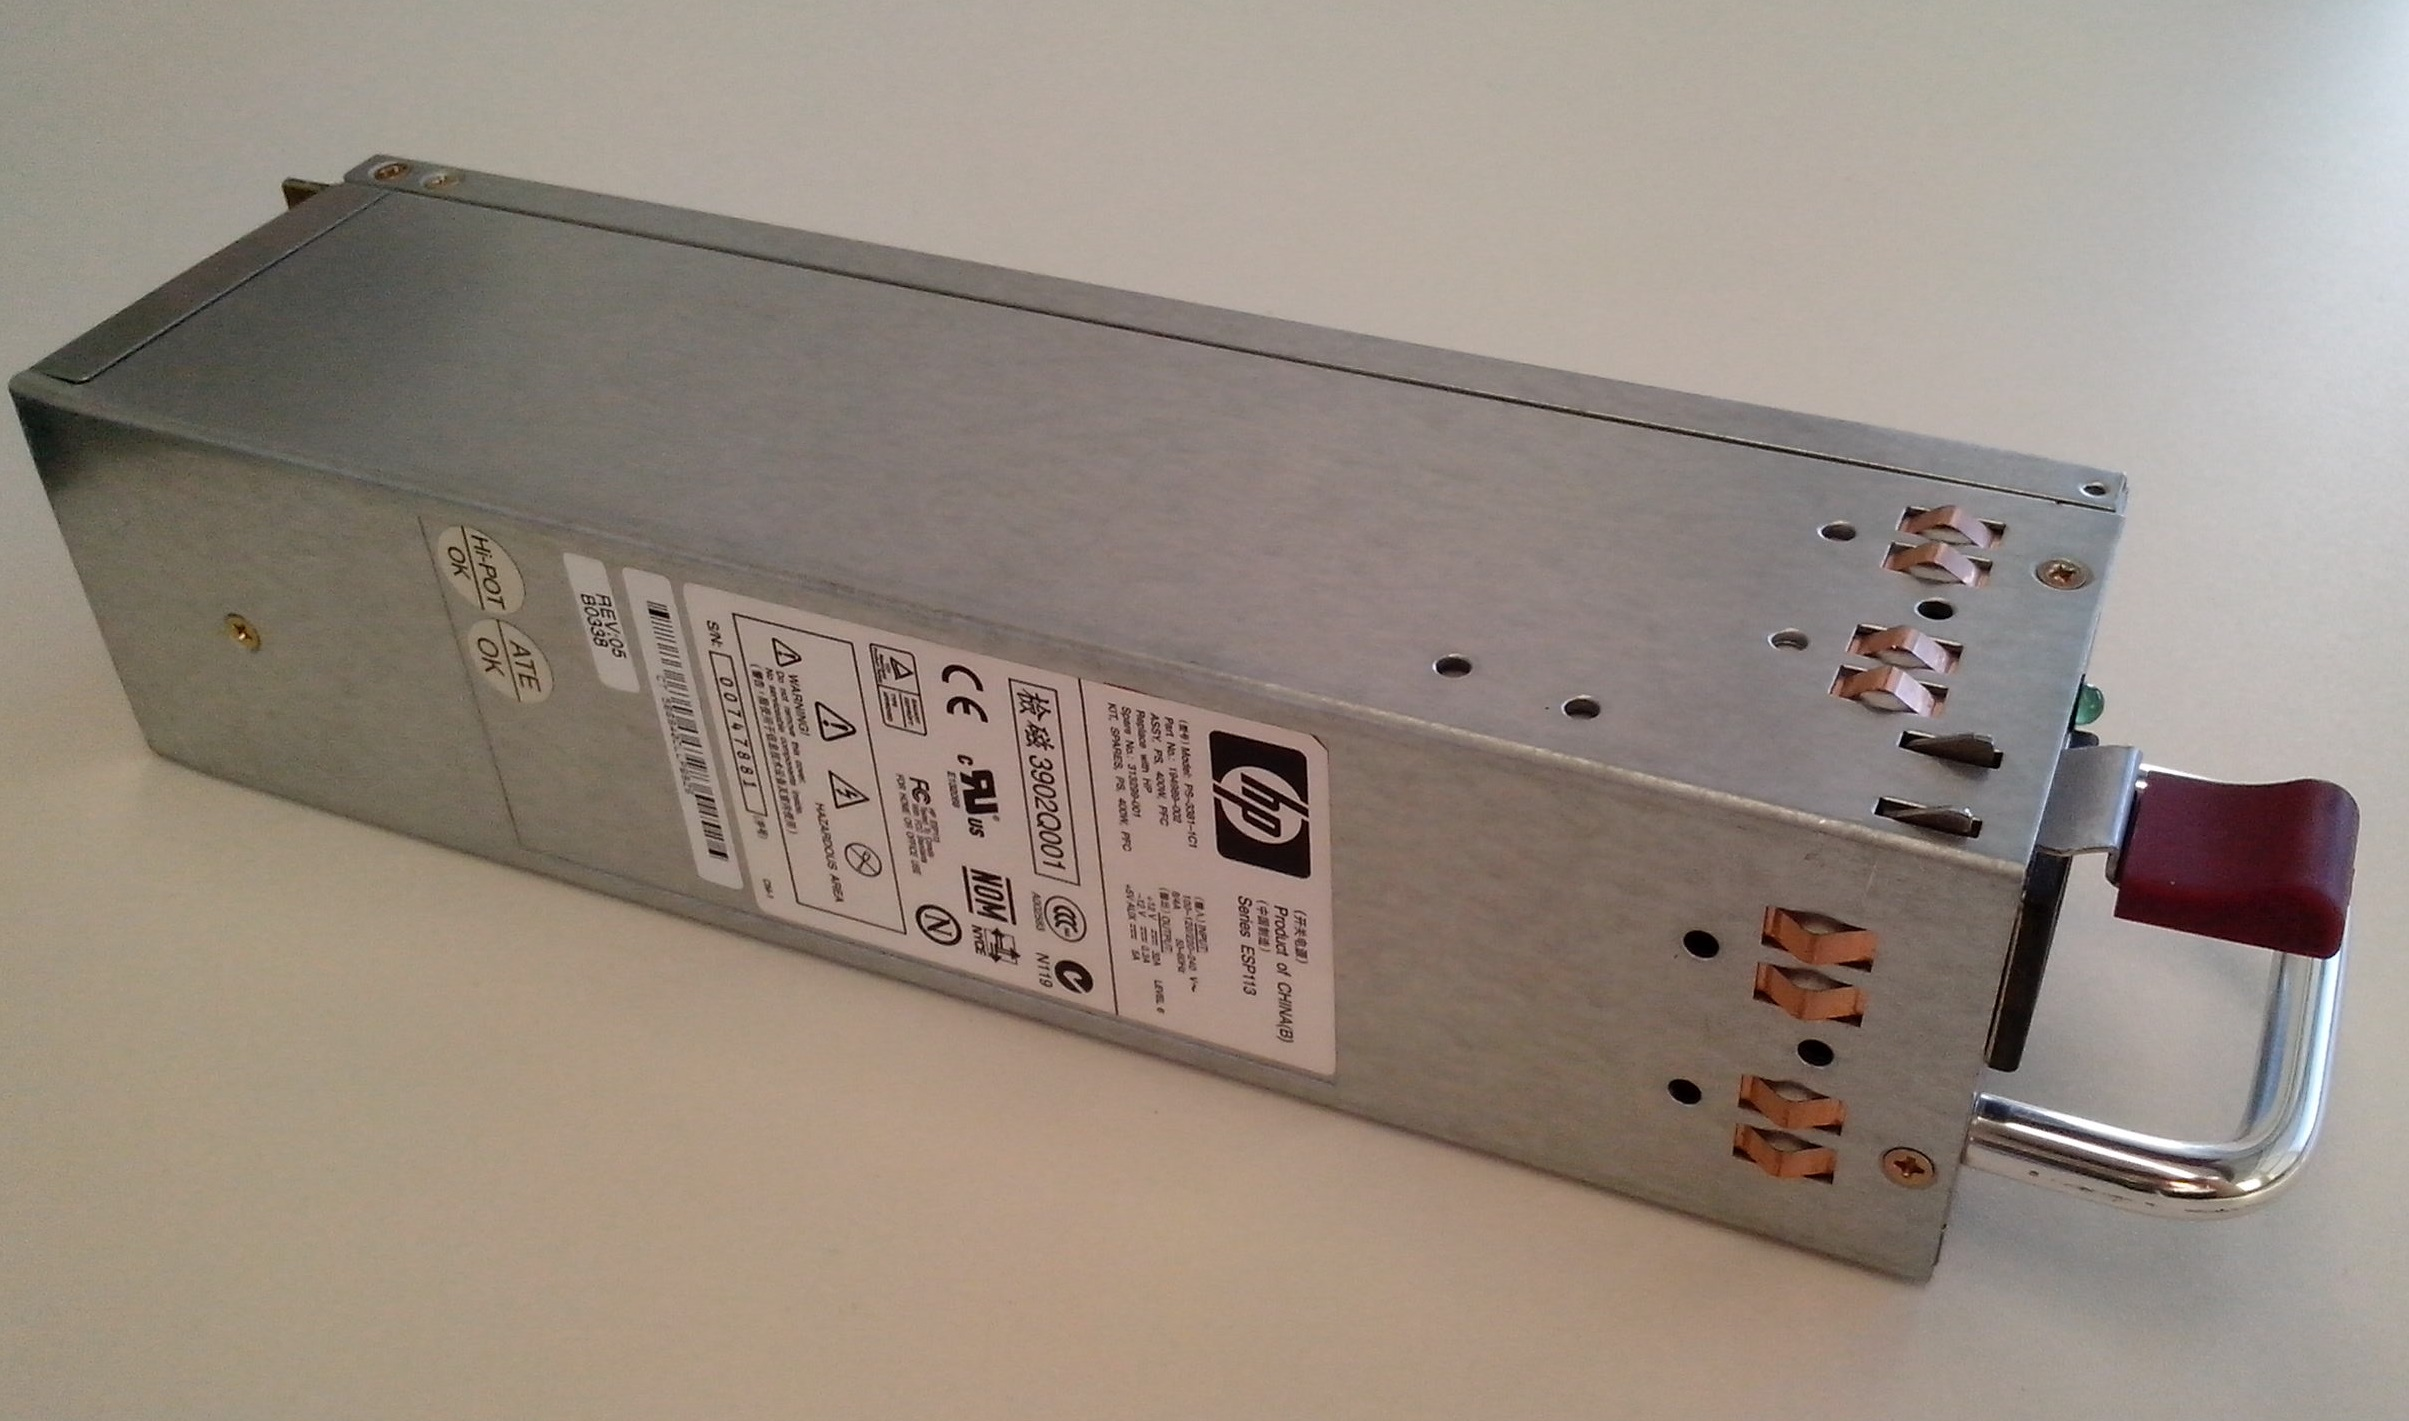
\includegraphics[width=0.5\textwidth]{../../fig/netzteil.jpg}
	\caption{HP Server Netzteil, PS-3381-1C1, 12V, 32A}
	\label{fig:server-power}
\end{figure}
